\setcounter{chapter}{6}
\chapter{Energies en mécanique}

\section{Travail d'une force}
\subsection{Cas général}

\blocrouge{Définition}{On considère une force $\vec{F}$ dont le point d'application se déplace de A vers B. Le déplacement est représenté par le vecteur $\vec{AB}$. L'énergie transférée au système par la force $\vec{F}$ pendant le déplacement $\vec{AB}$ s'appelle le travail de $\vec{F}$ il a pour expression: $$W(\vec{F}) = \trou{\vec{F}\cdot \vec{AB}} = F \times AB \times \trou{\cos(\alpha)}$$
Unités: W en J ; F en N ; AB en m
}

\etiquetterouge{Cas particuliers importants}
\begin{itemize}
	\item Si $\vec{F}$ est \trou{perpendiculaire} au déplacement alors $W(\vec{F})=0$
	\item Si $\vec{F}$ a même direction et \trou{même sens} que le déplacement $\vec{AB}$ alors $W(\vec{F})=F.AB>0$. La force aide au déplacement, le travail est \trou{moteur}.
	\item Si $\vec{F}$ a même direction et sens opposé au déplacement $\vec{AB}$ alors $W(\vec{F})=\trou{ - F.AB<0}$. La force résiste au déplacement, le travail est \trou{résistant}.
\end{itemize}

\etiquette{Exemples} Rédiger un exemple pour chacune des 3 situations. \vspace{5cm}

\subsection{Cas particuliers importants }
\etiquette{Vocabulaire} Qu'est-ce qu'une \textbf{force conservative } ?\\
\begin{itemize}
	\item Une force est conservative si son travail entre A et B ne dépend pas du chemin suivi pour aller de A à B. 
	\item Le poids et la force électrique sont des forces conservatives. 
\end{itemize}


Ainsi pour calculer le travail du poids on a uniquement besoin de la différence d'altitude entre A et B.

\blocrouge{Travail du poids}{

 Soit $h$ la différence d'altitude (dénivelé) entre A et B. On a $h=|z_A-z_B|$
\begin{itemize}
	\item Si le système descend en se déplaçant de A vers B: $W(\vec{P})=\trou{+mgh}$
		\item Si le système monte en se déplaçant de A vers B: $W(\vec{P})=\trou{-mgh}$ 
\end{itemize}

 Ce qui s'écrit de manière plus générale: $$W_{A\rightarrow B}(\vec{P})  = \trou{mg(z_A-z_B)}$$}
 
 \begin{center}
 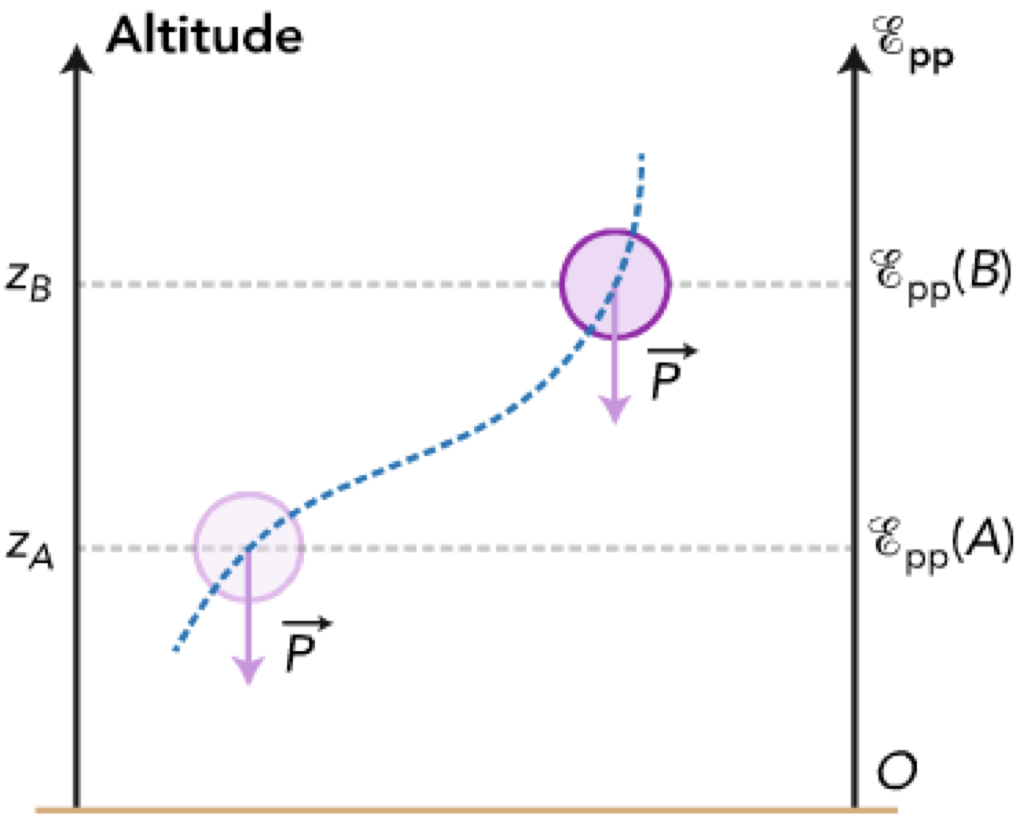
\includegraphics[scale=.4]{figures/travail_poids.png}	
 \end{center}
 
 

\blocrouge{Travail de la force électrique}{
La force électrique $\vec{F}=q\vec{E}$ est une force conservative. On retiendra que lorsqu'une charge $q$ se déplace de A vers B dans un champ électrique $\vec{E}$ son travail s'écrit: $$W(\vec{F})=\vec{F}\cdot\vec{AB} = \trou{q\times U_{AB}}$$
Unités: W en J ; q en C et $U_{AB}$ en V

}

\etiquette{Remarque} Dans les exercices, A et B désigneront généralement les plaques chargées entre lesquelles il existe un champ électrique $\vec{E}$. $U_{AB}$ est alors la tension entre ces plaques. Voir \textbf{livre p 245.}
\section{Théorème de l'énergie cinétique}
\subsection{Énoncé}
\blocrouge{Théorème de l'énergie cinétique}{La variation d'énergie cinétique d'un système qui se déplace d'un point A vers un point B est égale à la somme des \trou{travaux des forces} sur le trajet AB.$$Ec(B) - Ec(A) = \Sigma W_{A\rightarrow B}(\overrightarrow{F})$$
Cette année le système subit en général une force seule qui travaille il n'y aura pas de somme à effectuer. cf exercice
}
\subsection{Applications}

 \etiquette{Application 1}

On se place dans le cas d'une balle lâchée (sans vitesse initiale)  d'une hauteur  $h=5$ m. A l'instant $t_1=0$ s, la balle est lâchée et à l'instant $t_2$ elle touche le sol.
\begin{enumerate}
	\item Faire un schéma.
	\item Calculer le travail du poids pendant la chute.
	\item Ecrire le théorème de l'énergie cinétique et en déduire la valeur de la vitesse de la balle lorsque celle-ci atteint le sol.
\end{enumerate}


 \etiquette{Application 2}

 Une bille de masse m=50 g roule sur un support parfaitement glissant. Elle est lancée au point O à une vitesse de 4 m/s. Sur le trajet OA le support est parfaitement horizontal. Le trajet AB est incliné de $\SI{20}{\degree}$. Au point B, la bille rebrousse chemin puis commence à redescendre la pente. 

 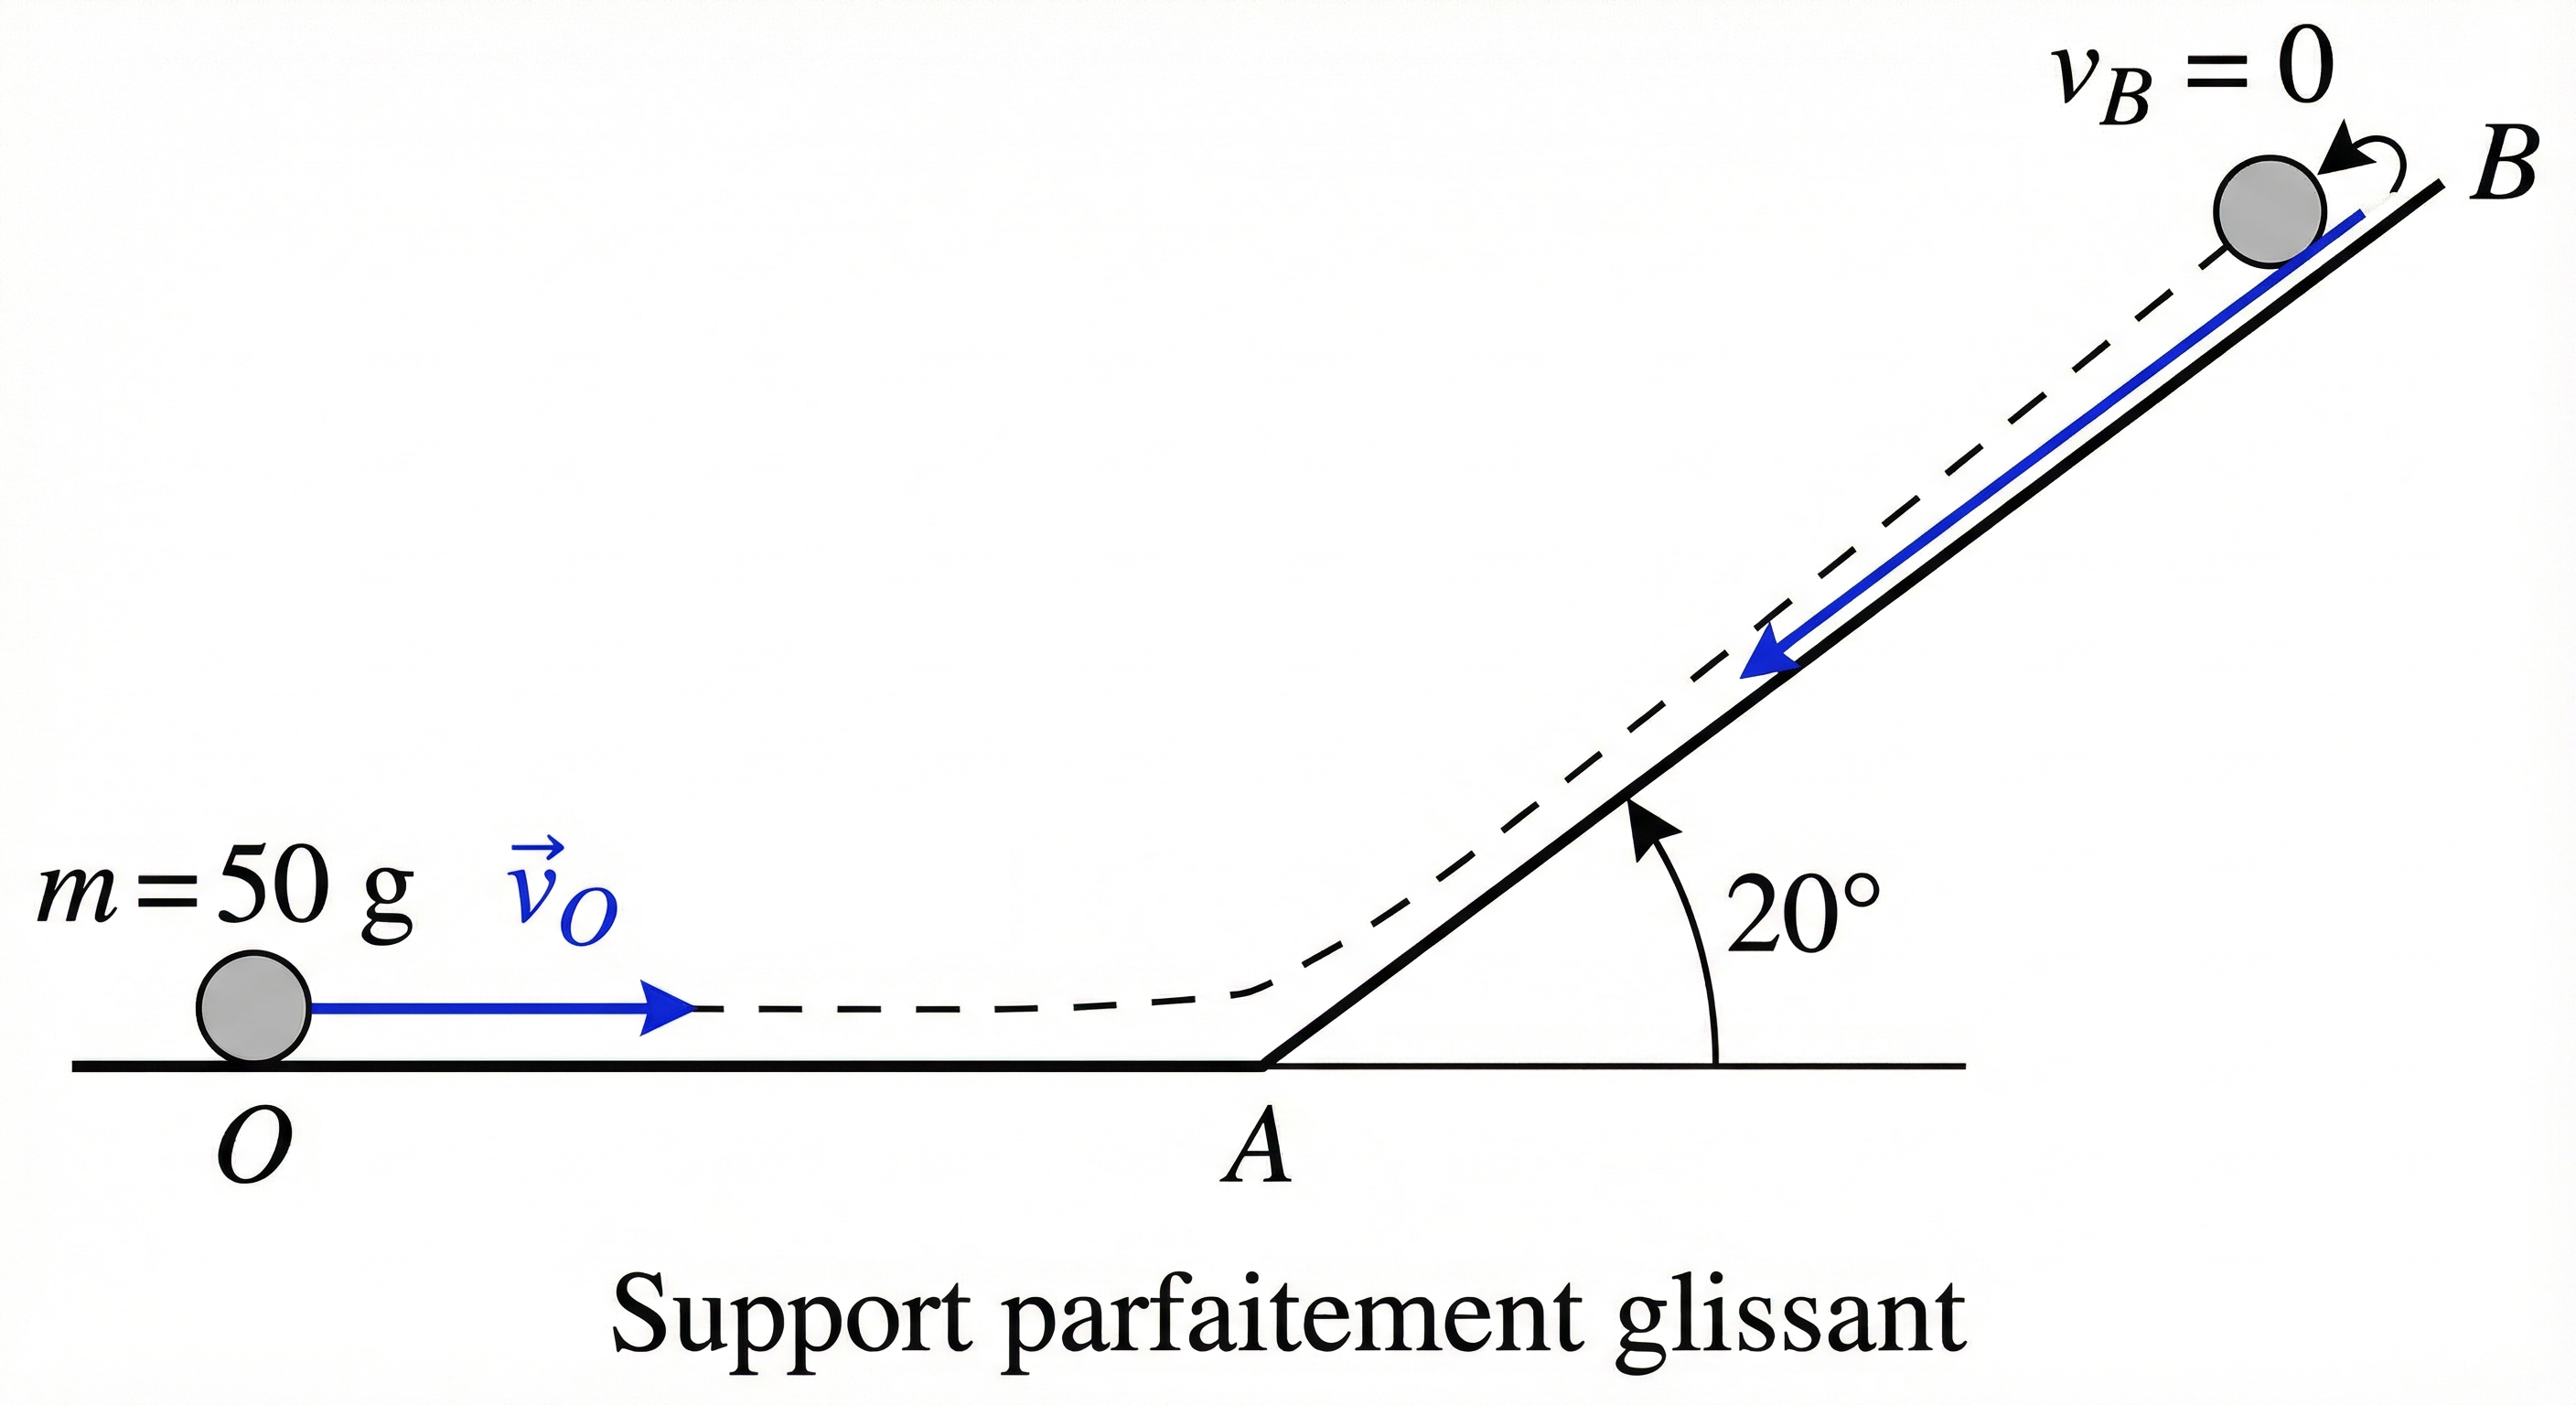
\includegraphics[width=10cm]{figures/fig_exo_energie.png}

 \begin{enumerate}

 	\item Faire le bilan des forces s'exerçant sur la bille.
 	\item Calculer les travaux des forces sur le trajet OA.
 	\item En utilisant le théorème de l'énergie cinétique, justifier que la vitesse de la bille en A est aussi de 4m/s.
 	\item Calculer la variation d'énergie cinétique entre A et B.
 	\item En déduire la valeur du travail du poids sur le trajet AB. 
 	\item Déterminer la distance AB.
 \end{enumerate}

 \etiquette{Application 3} Etude énergétique de l'accélération d'une particule chargée

On considère un proton initialement au repos en un point O. Ce proton est soumis au champ électrique $\vec{E}$ voir schéma. Les deux plaques sont soumises à une tension de 2,00 MV. Les plaques sont distantes de d=10,0 cm. 

\begin{center}
	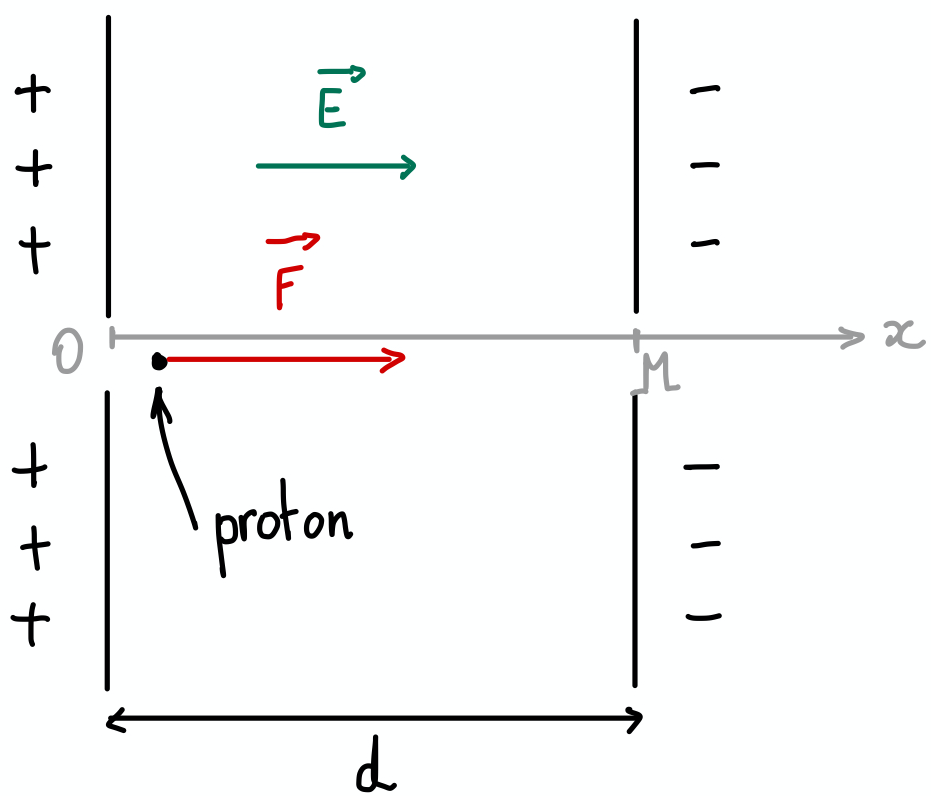
\includegraphics[height=4.5cm]{figures/dynamique/accelerateur_lineaire.png}

\end{center}


\etiquette{Objectif} Calculer la vitesse du proton au point M

\textbf{Plan de travail}
\begin{enumerate}
	\item Calculer le travail de la force électrique sur le déplacement de O vers M.
	\item Ecrire le théorème de l'énergie cinétique.
	\item Isoler la vitesse en M dans l'équation du théorème de l'énergie cinétique
\end{enumerate}

\textbf{Aides}
\begin{enumerate}
	\item 
	Utiliser la définition de la force électrique. Utiliser la définition du travail de la force sur le trajet $\vec{OM}$ $$W(\vec{F}) = \vec{F}  \cdot \overrightarrow{OM}$$ Le produit scalaire de deux vecteurs colinéaires et de même sens est égal au produit de leurs normes.
	\item $\Delta Ec = W(\vec{F})$
	\item $\Delta Ec = \frac{1}{2}mv_M^2$ et finalement $v_m= \sqrt{\frac{2qU}{m} }$
\end{enumerate}

\blocrouge{Travail personnel}{
\begin{itemize}
	\item Ex 24 et 25 p 254 et suivantes
	\item 2023 Réunion Sciences physiques pour les Sciences de l'ingénieur.e Jour 1 Lien: \url{https://www.labolycee.org/le-scanner-rayons-x}
	\item Vidéo présentant un exercice type bac:\\ \url{https://www.youtube.com/watch?v=LSX_AUg_MNQ}
	\item Imprimante à jet d'encre continu \\ \url{https://www.labolycee.org/imprimante-jet-dencre-continu}
	\end{itemize}
}
